\title[Introducing Madagascar]{Introducing Madagascar \\
{\small A Computational Platform for Geophysical Data Processing and 
Reproducible Numerical Experiments}}

\author[S. Fomel] % (optional, nur bei vielen Autoren)
{Sergey~Fomel\inst{1} \and Paul~Sava\inst{2} \and Felix Herrmann\inst{3}}
% - Der \inst{?} Befehl sollte nur verwendet werden, wenn die Autoren
%   unterschiedlichen Instituten angeh�ren.

\institute[UT Austin] % (optional, aber oft n�tig)
{
  \inst{1}%
  Bureau of Economic Geology \\
  Jackson School of Geosciences \\
  University of Texas at Austin
  \and
  \inst{2}%
  Colorado School of Mines \\
  \inst{3}%
  University of British Columbia
}

\date[EAGE Open-Source Software]{June 11, 2006}

\setbeamercolor{quotecol}{fg=white,bg=black}

\newcommand{\quotebox}[3]{
  \begin{beamercolorbox}[wd=\textwidth,center]{quotecol}
    \begin{quote}
      #1 \\ 
      \color{yellow}{\emph{#2}, #3}
    \end{quote}
    \end{beamercolorbox}
}

\begin{frame}
  \titlepage
\end{frame}

\begin{frame}
\frametitle{From RSF to Madagascar}
\begin{minipage}{0.55\textwidth}
\vfill
\begin{center}
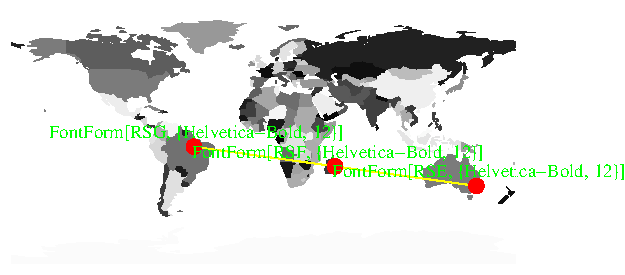
\includegraphics[width=\textwidth]{Math/Fig/rsf}
\end{center}
\vfill
\end{minipage}
\hfill
\begin{minipage}{0.35\textwidth}
\begin{center}
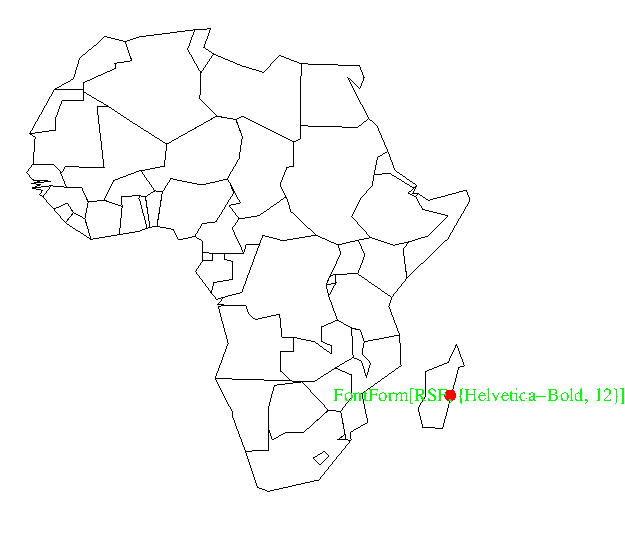
\includegraphics[width=\textwidth]{Math/Fig/africa}
\end{center}
\end{minipage}
\end{frame}

\begin{frame}
  \frametitle{Outline}
  \tableofcontents[pausesections]
\end{frame}

\section{New}
\begin{frame}<beamer>
  \frametitle{Outline}
  \tableofcontents[currentsection]
\end{frame}

\begin{frame}
  \frametitle{History}
  \begin{itemize}
  \item Started in June 2003
  \item 6 main contributors
  \item Version 0.9 released June 2006
  \item Development version
    \begin{itemize}
    \item 2,000 revisions
    \item 300 main programs (140,000 lines of C) 
    \item 3,000 tests (40,000 lines of Python)
    \item 30 papers (20,000 lines of \LaTeX)
    \end{itemize}
  \item \url{http://rsf.sf.net/}
  \end{itemize}
\end{frame}

\begin{frame}
  \frametitle{Heritage}
  \begin{itemize}
  \item SEPlib
    \begin{itemize}
    \item Rob Clayton, Jon
      Claerbout, Dave Hale, Stew Levin, Rick Ottolini, Joe Dellinger, Steve
      Cole, Dave Nichols, Martin Karrenbach, Biondo Biondi, Bob Clapp
    \end{itemize}
  \item SEP reproducible research system
    \begin{itemize}
    \item  Martin Karrenbach, Matthias Schwab, Joel Schroeder, Sergey Fomel, 
    Bob Clapp
    \end{itemize}
  \item Seismic Unix
  \item DDS
  \end{itemize}
\end{frame}

\section{Test Driven Development}
\begin{frame}<beamer>
  \frametitle{Outline}
  \tableofcontents[currentsection]
\end{frame}

\begin{frame}
  \frametitle{Test Driven Development}
  \begin{itemize}
  \item XP, agile software engineering, refactoring
    \begin{itemize}
    \item Tests drive development
    \end{itemize}
  \item Computational geophysics
    \begin{itemize}
    \item Tests are numerical experiments
    \end{itemize}
  \item Science
    \begin{itemize}
      \item Reproducible experiments mean \href{http://www.reproducibility.org/RSF/}{progress}
    \end{itemize}
  \end{itemize}
\end{frame}

\begin{center}
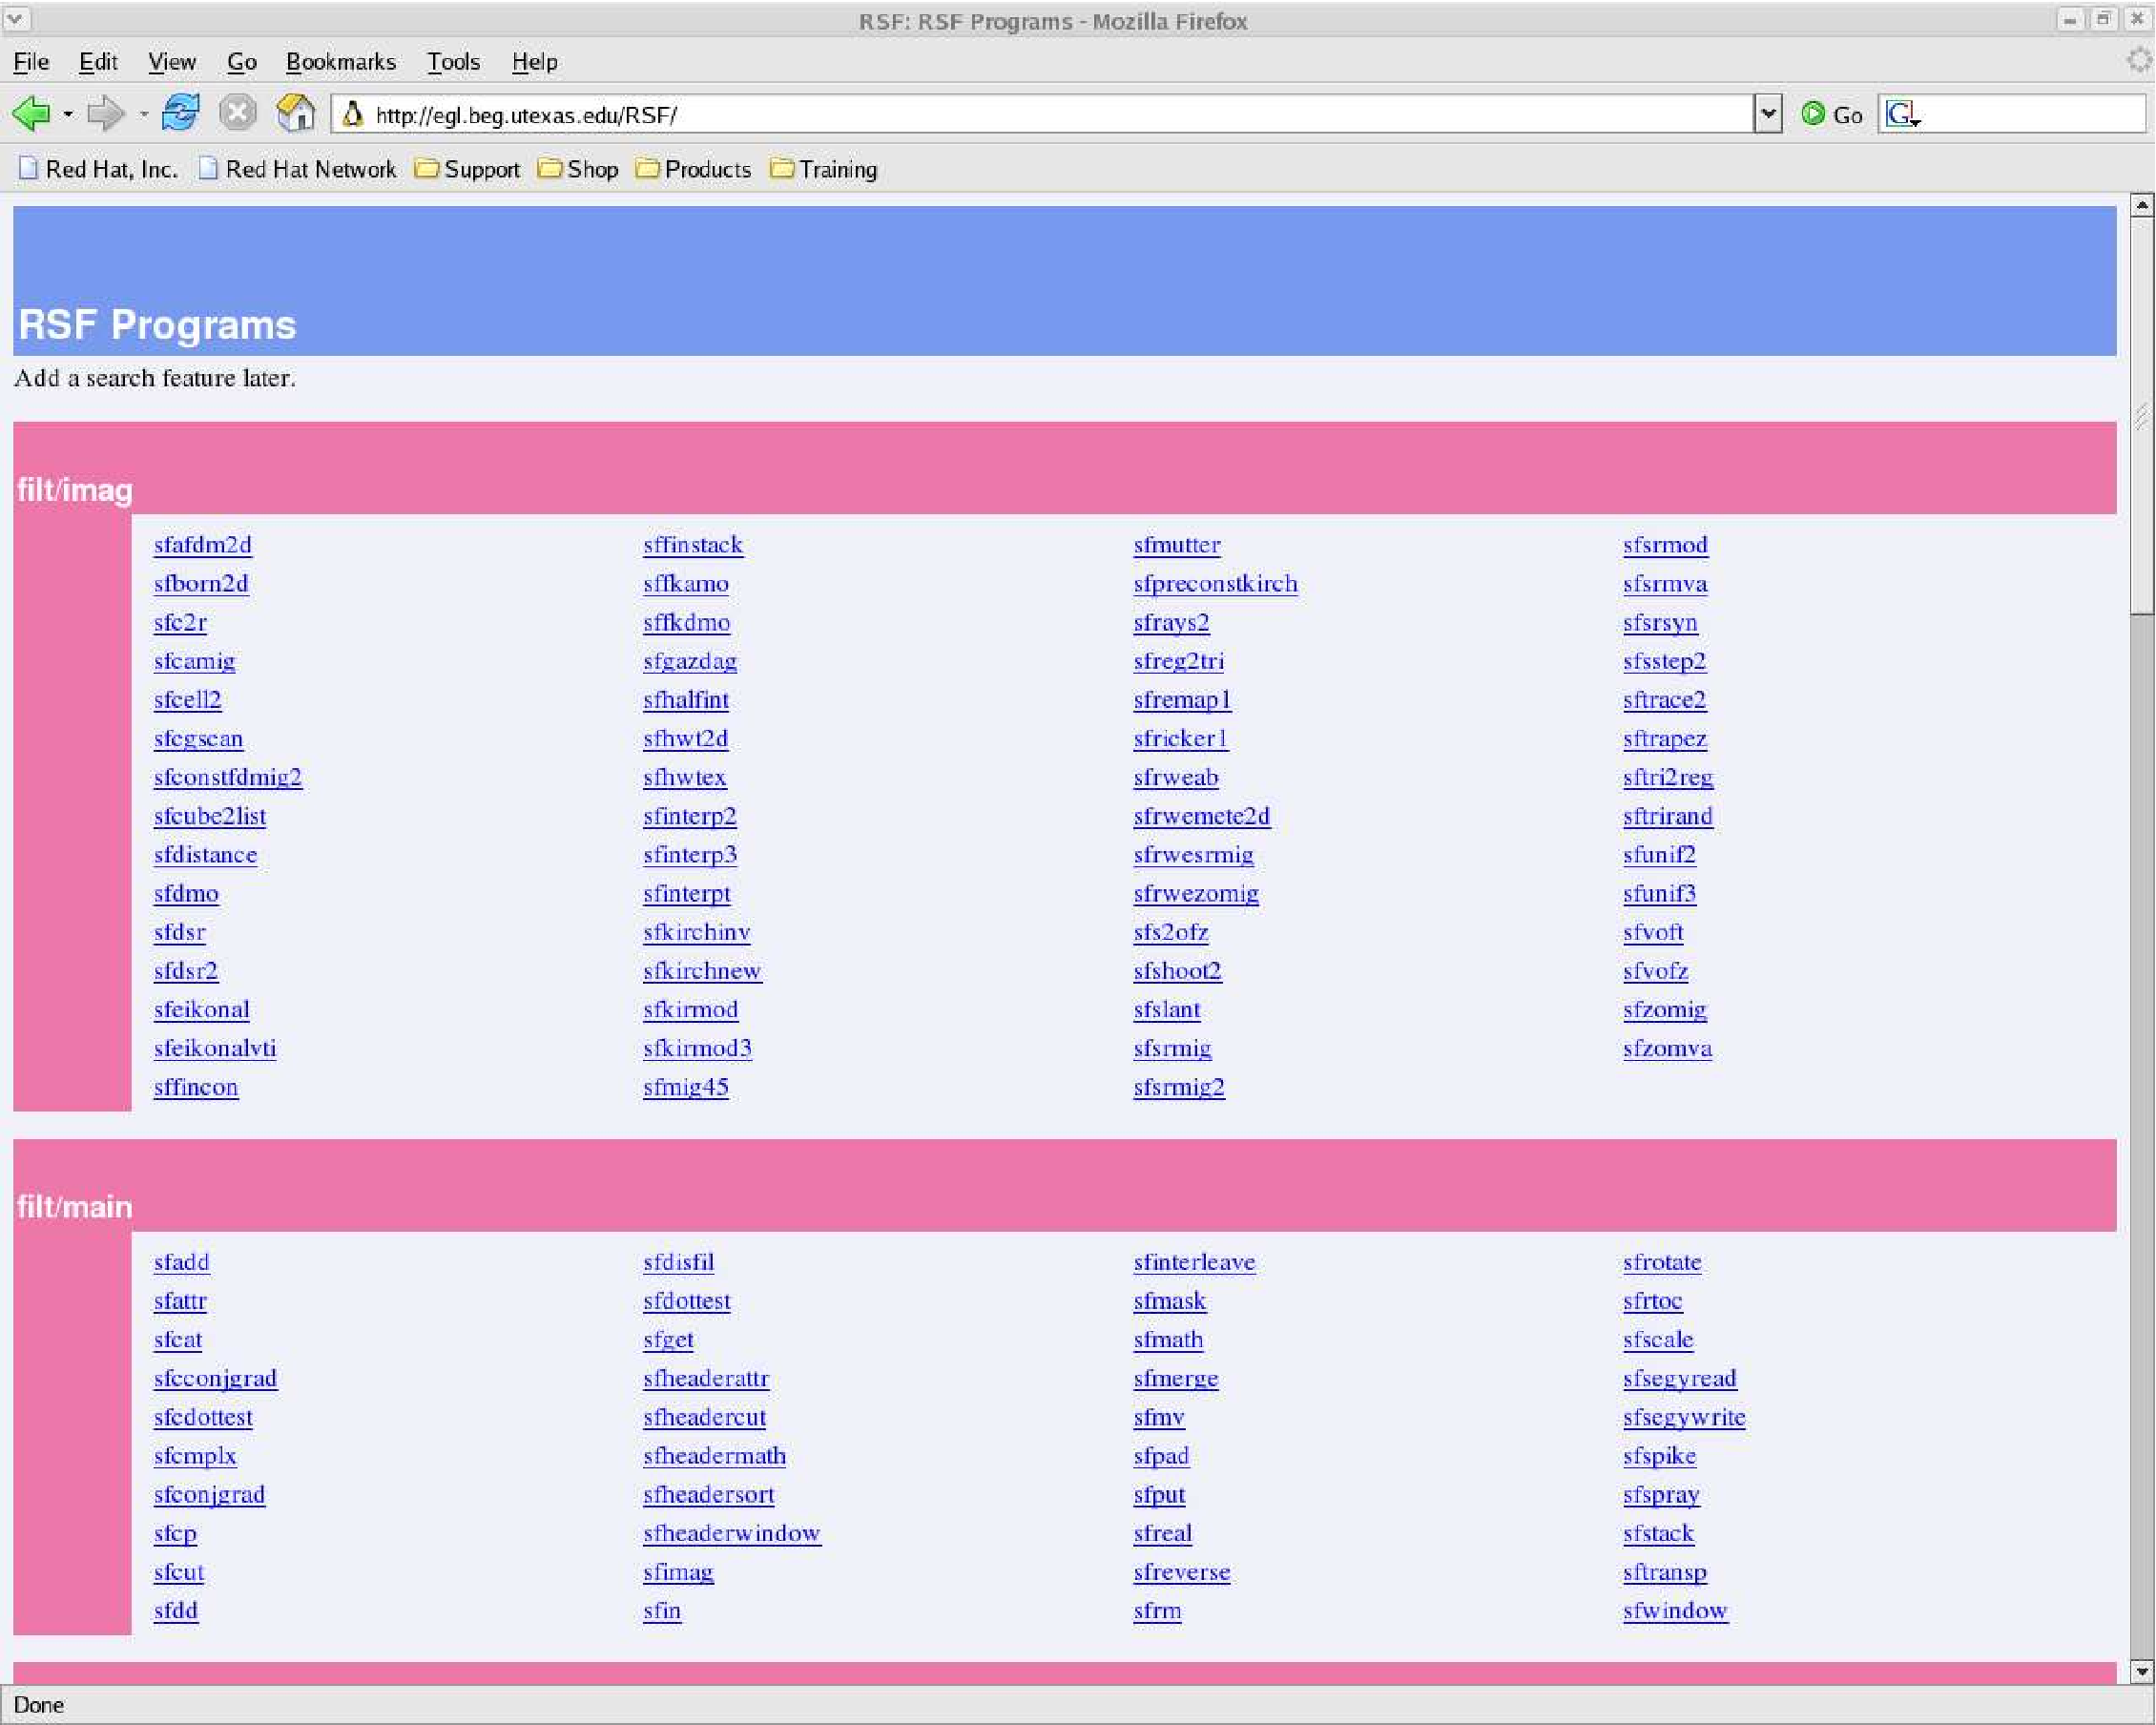
\includegraphics[height=\textheight]{Fig/rsf} \newpage
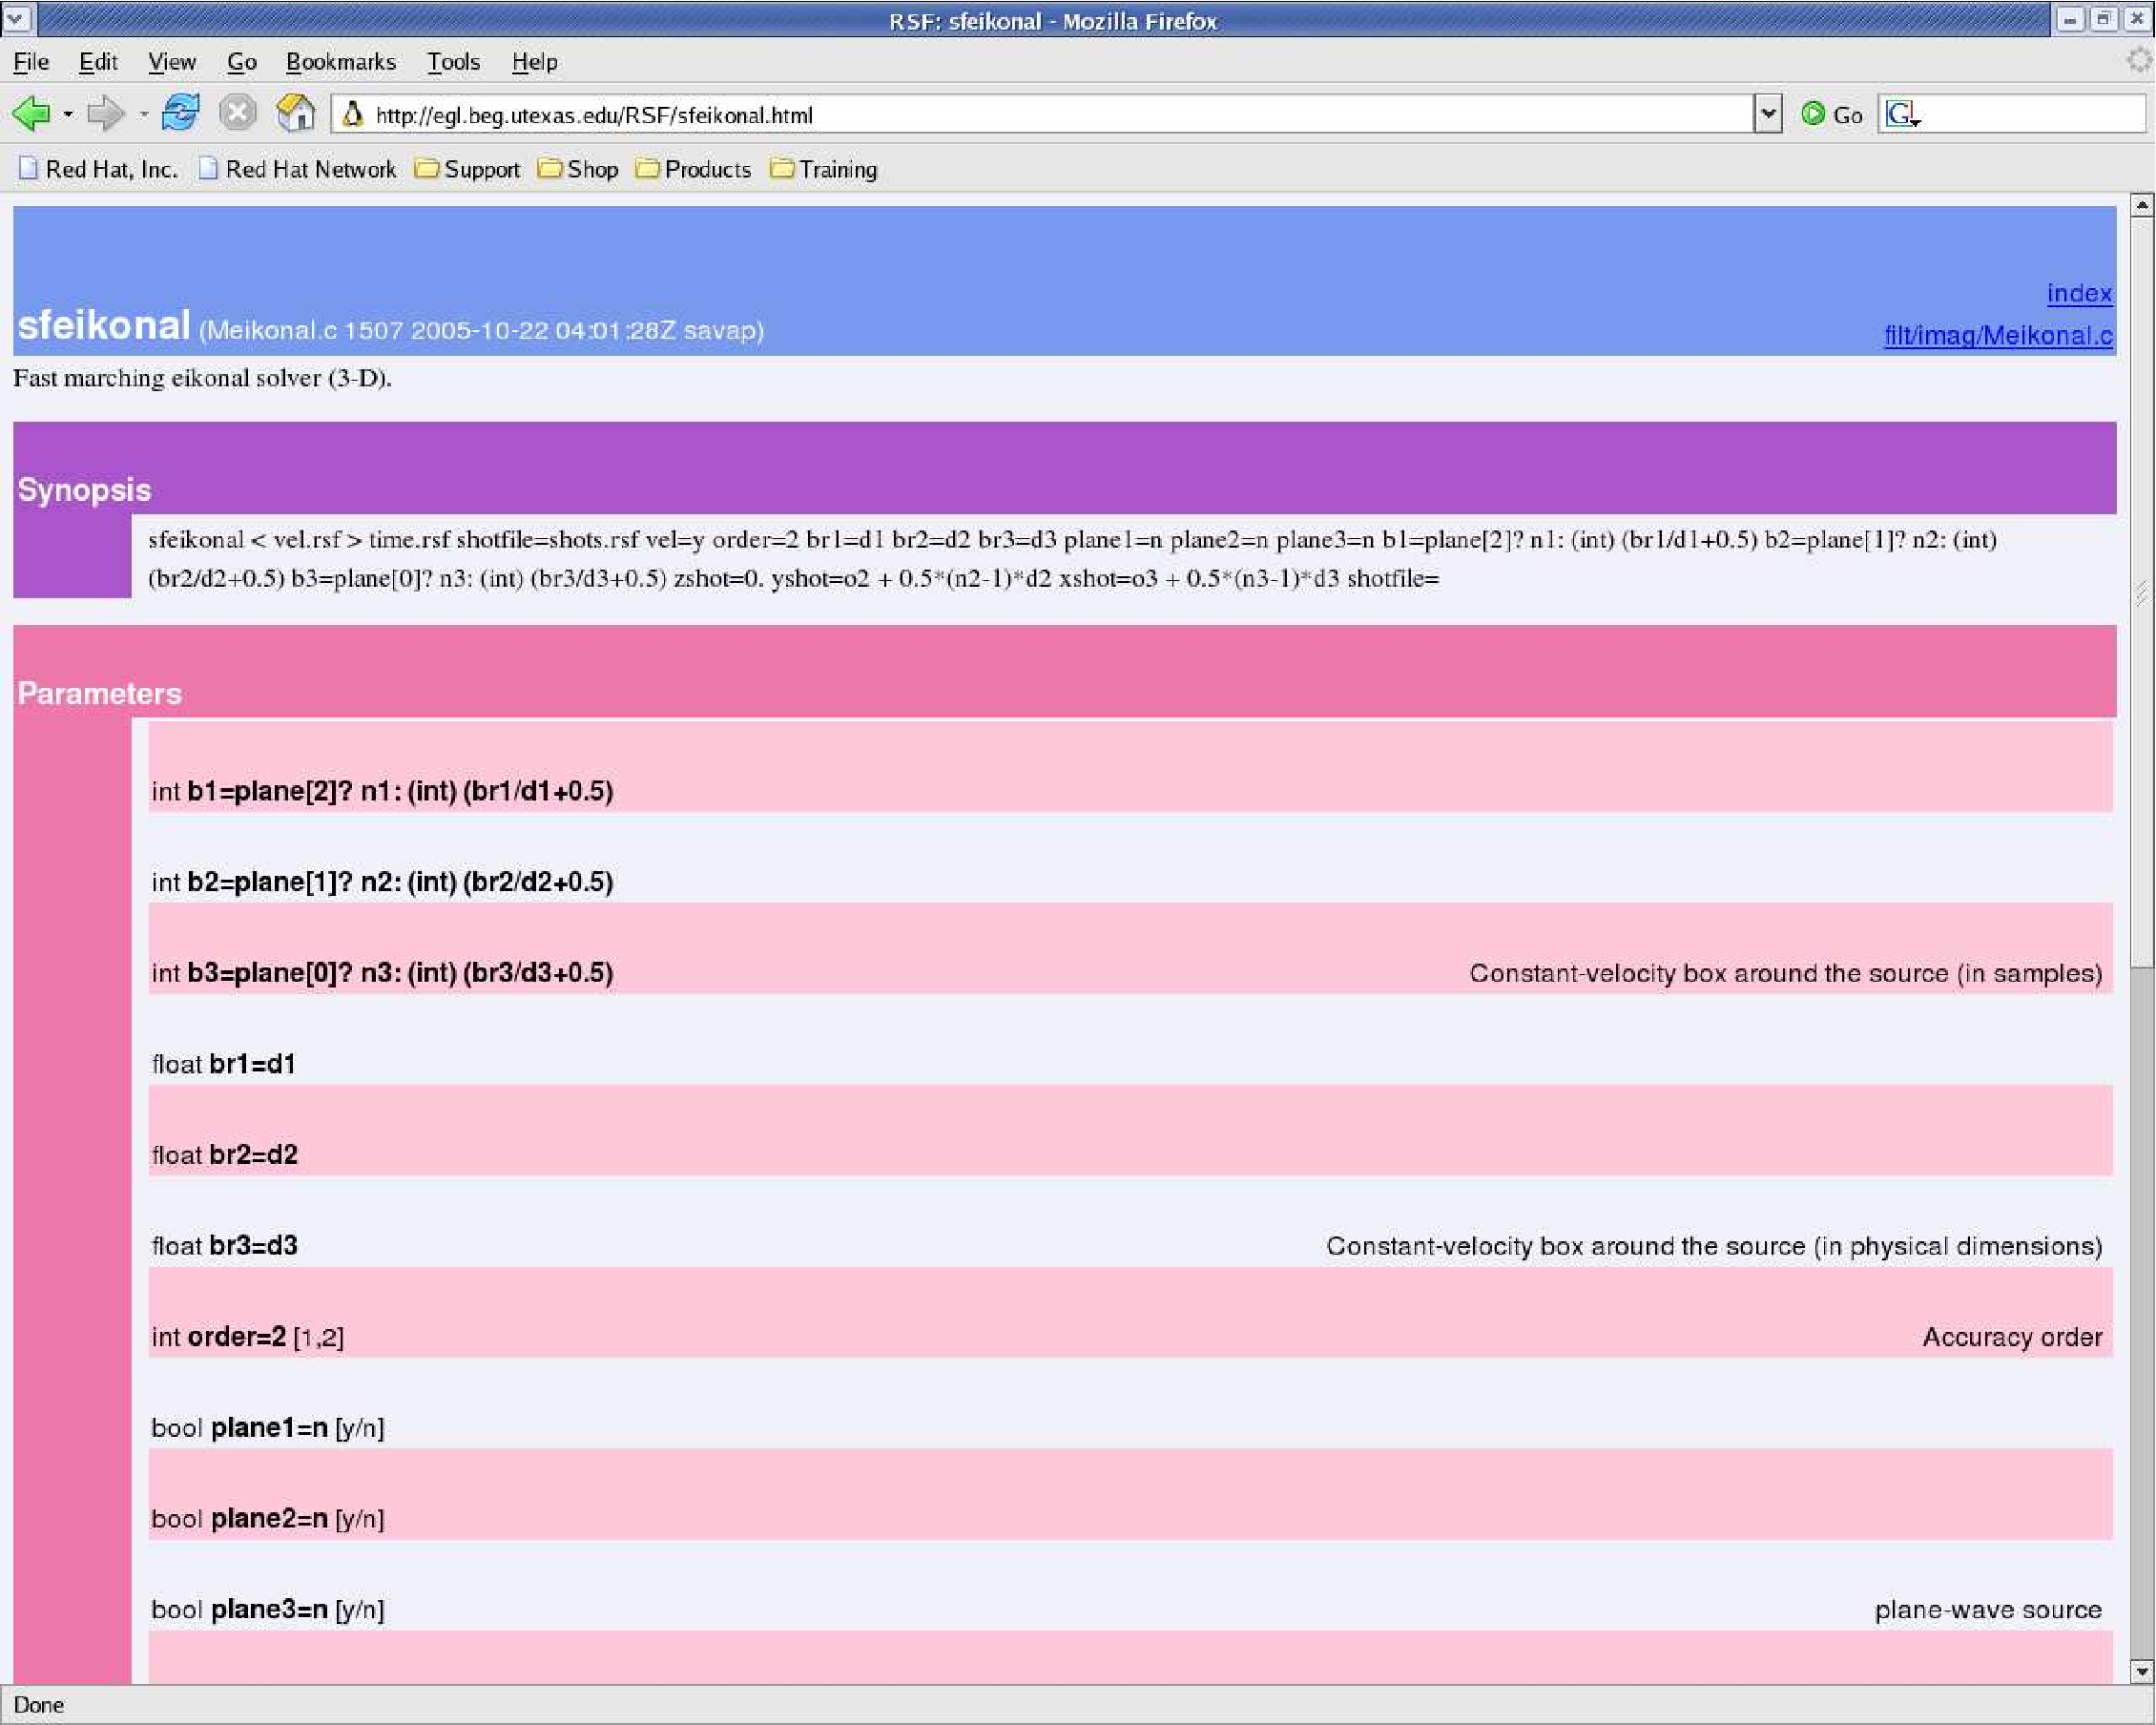
\includegraphics[height=\textheight]{Fig/eikonal1} \newpage
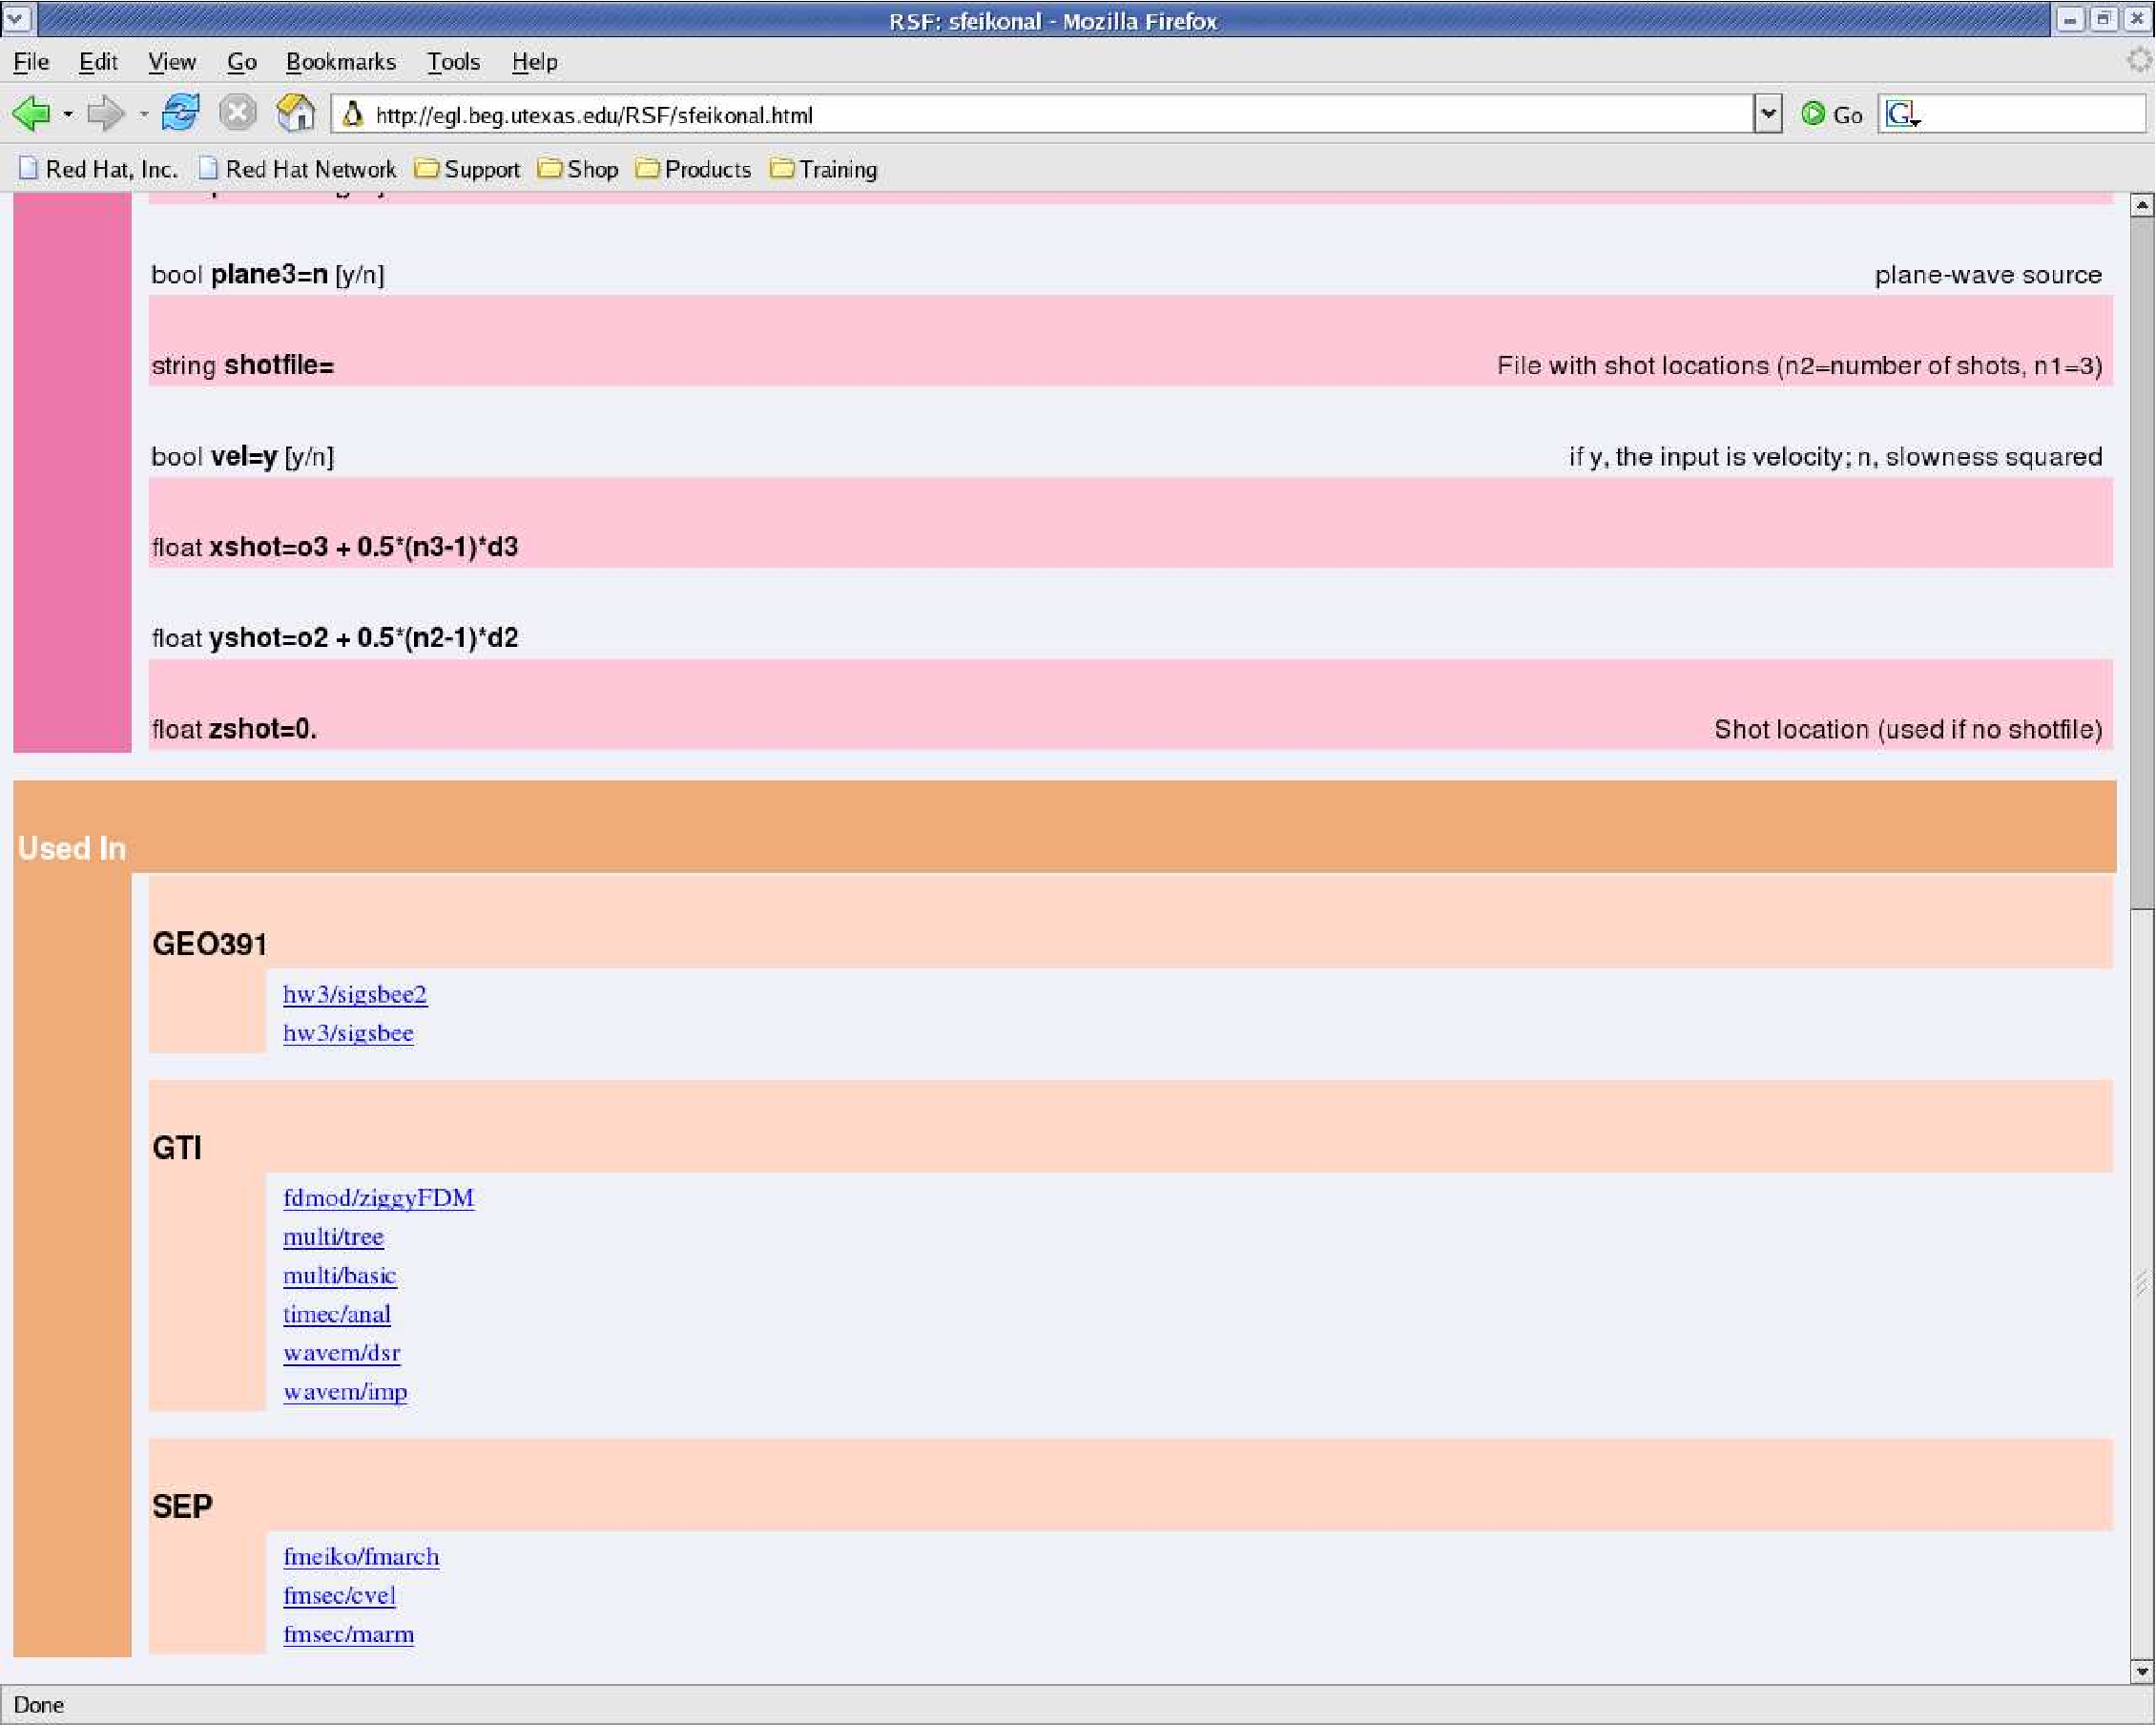
\includegraphics[height=\textheight]{Fig/eikonal2} \newpage
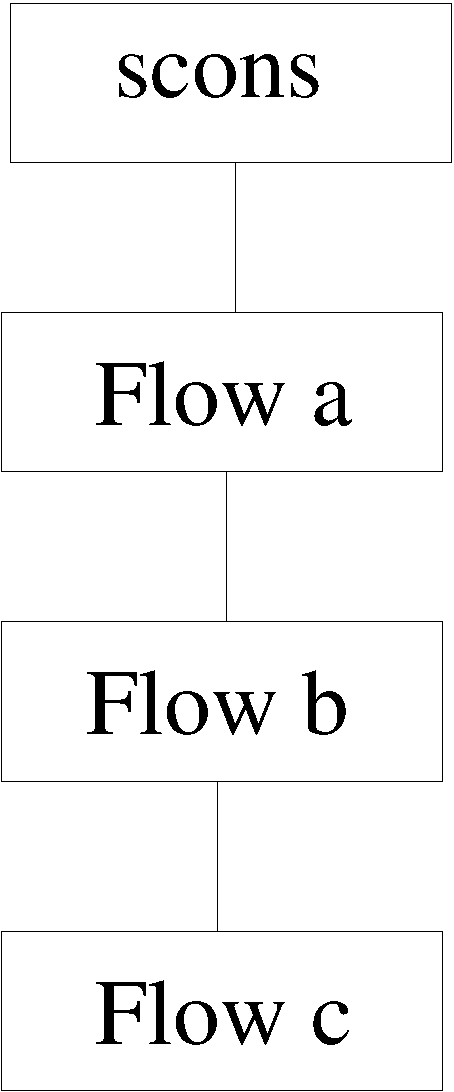
\includegraphics[height=\textheight]{Fig/scons} \newpage
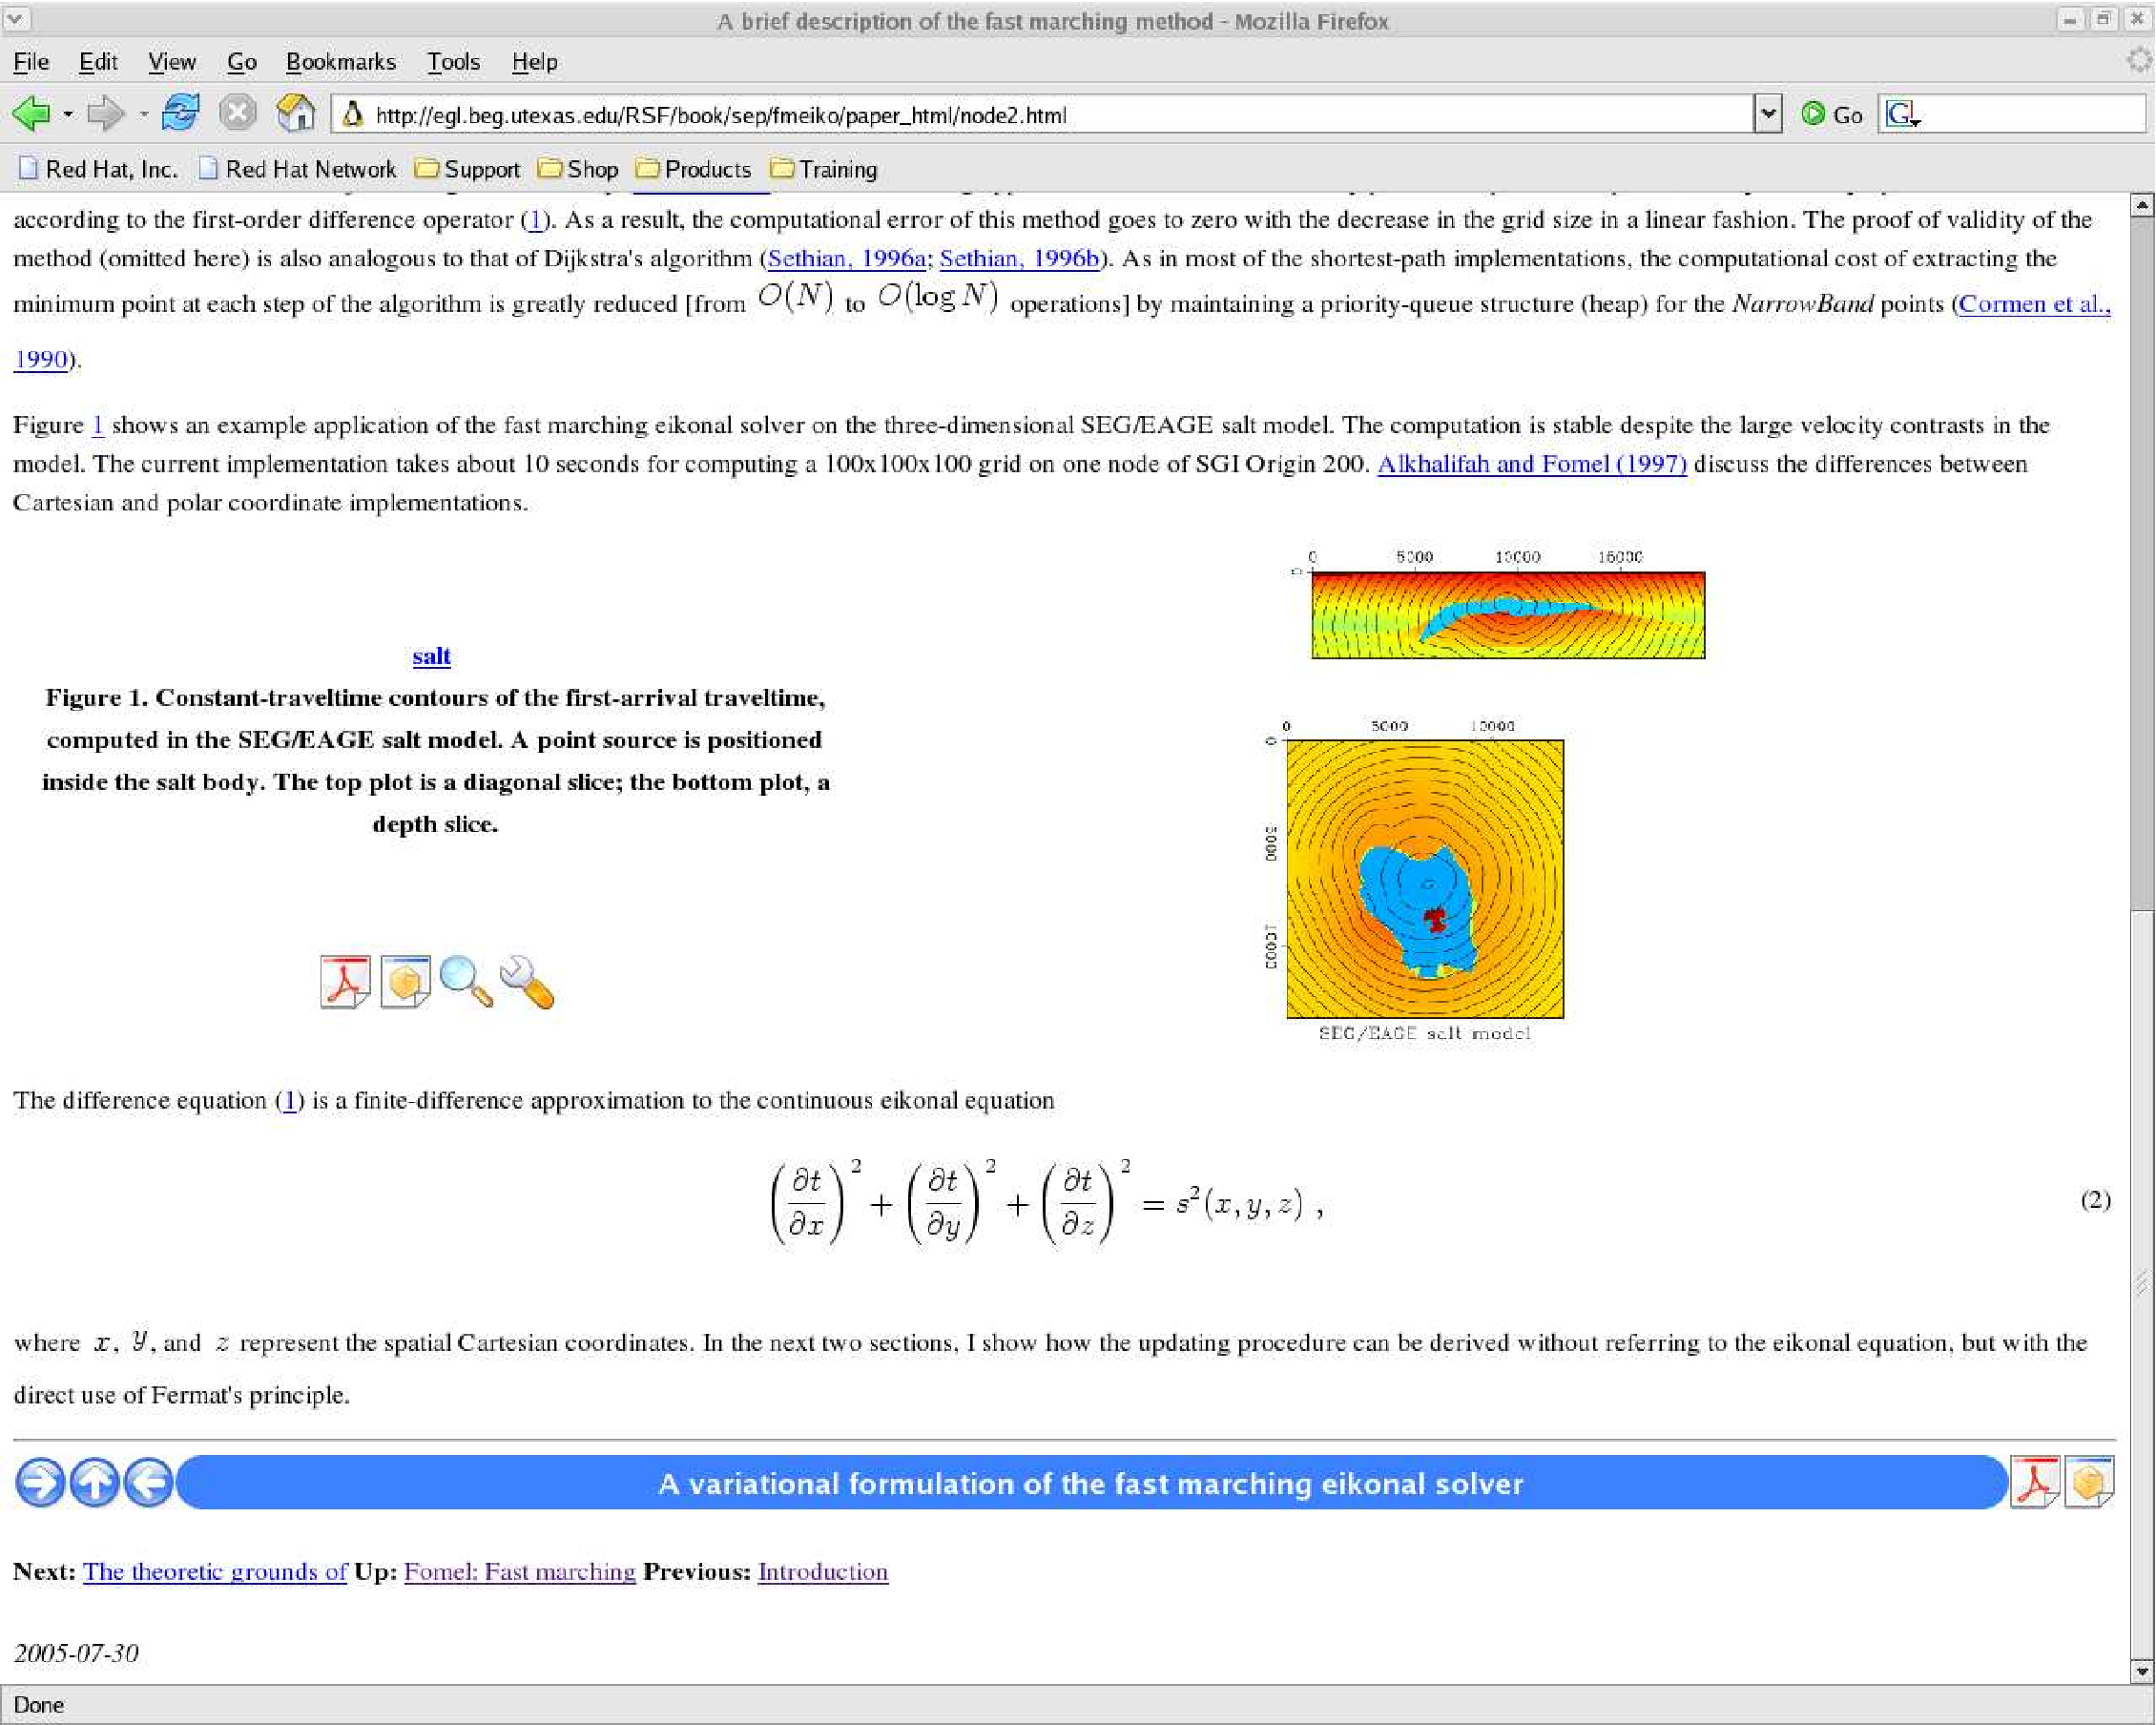
\includegraphics[height=\textheight]{Fig/salt} \newpage
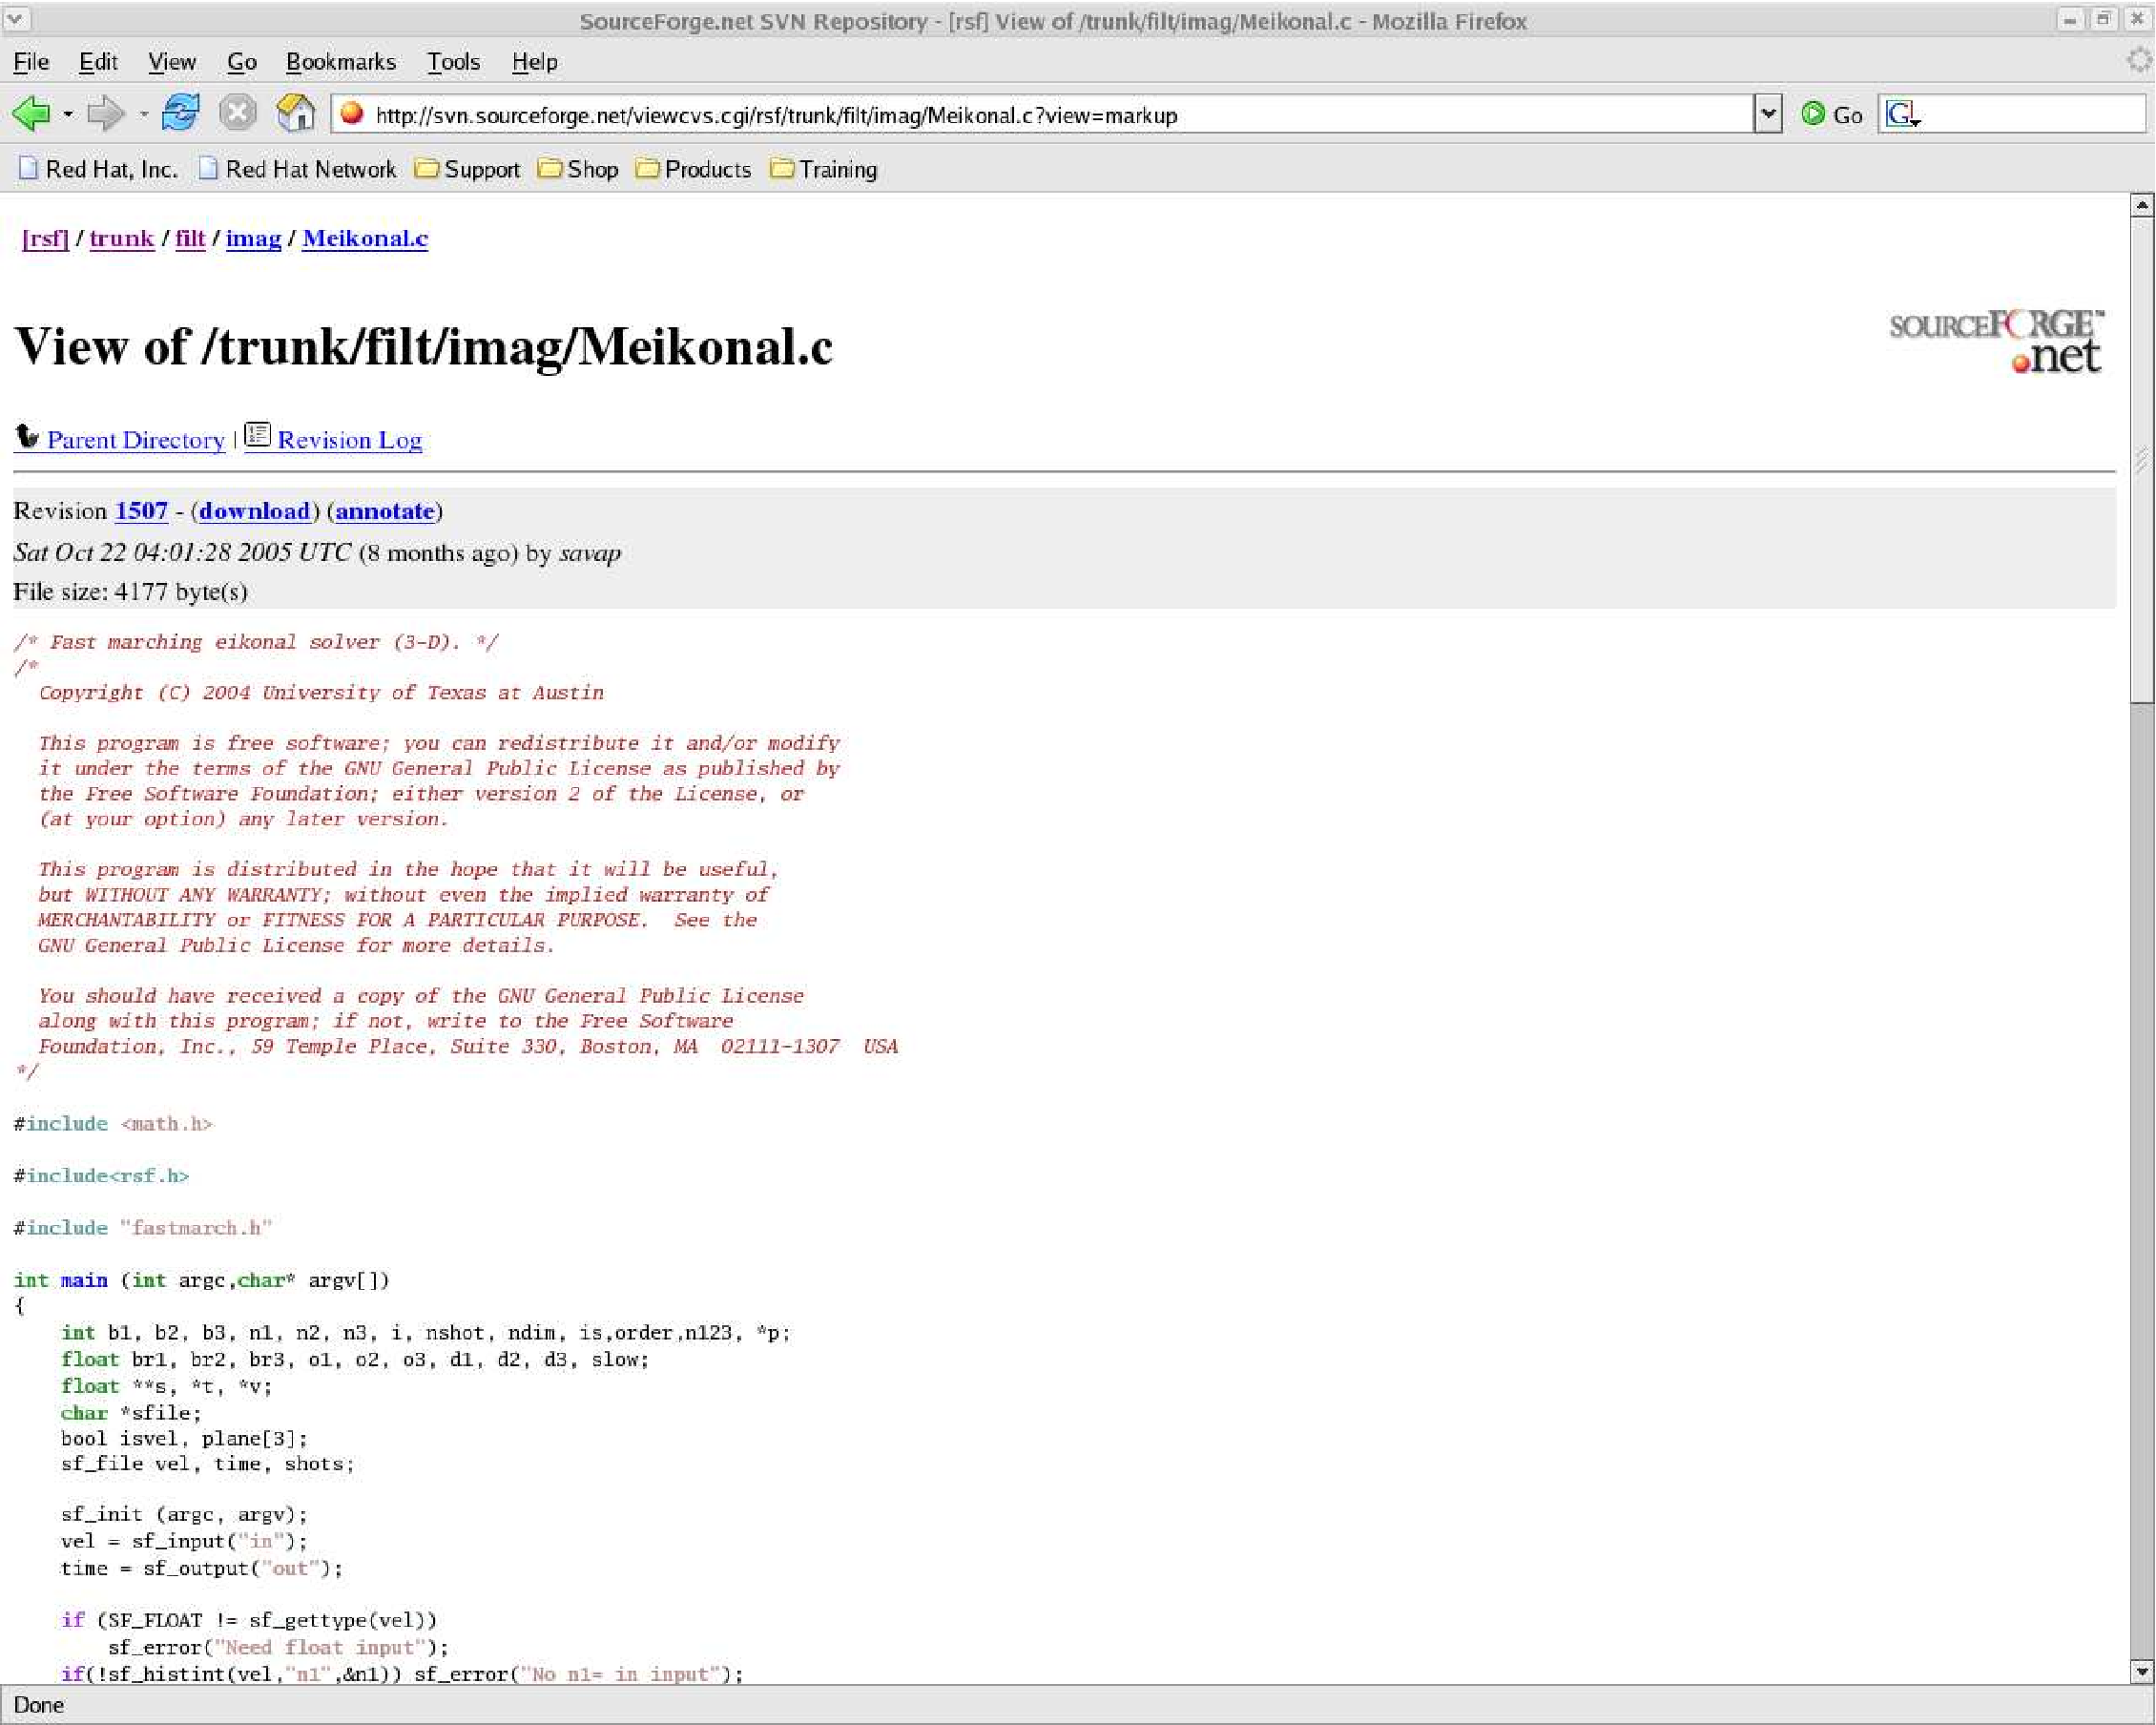
\includegraphics[height=\textheight]{Fig/code} \newpage
\end{center}

\begin{frame}
  \frametitle{Inspirational Quotes}
  \quotebox{Abandoning the habit of secrecy in favor of process
  transparency and peer review was the crucial step by which alchemy
  became chemistry.  In the same way, it is beginning to appear that
  open-source development may signal the long-awaited maturation of
  software development as a discipline.}
{Eric S. Raymond}{The art of UNIX programming, 2004}
\end{frame}

\begin{frame}
  \frametitle{Inspirational Quotes}
  \quotebox{
    The purpose of reproducible research is to facilitate someone going a step
    further by changing something. The first step that 
    someone will want to make
    is to be sure that your work is reproducible before they change and improve
    upon it.}{Jon F. Claerbout}{Reproducible research}
\end{frame}

\begin{frame}
  \frametitle{Inspirational Quotes}
  \quotebox{
An article about computational science in a scientific publication is not the
scholarship itself, it is merely advertising of the scholarship. The actual scholarship
is the complete software development environment and the complete
set of instructions which generated the figures.}
{Jon B. Buckheit and David L. Donoho}{WaveLab and reproducible research, 1995}
\end{frame}

\begin{frame}
  \frametitle{Inspirational Quotes} \quotebox{ 
Within the world of science, computation is now rightly seen as a
third vertex of a triangle complementing experiment and
theory. However, as it is now often practiced, one can make a good
case that computing is the last refuge of the scientific scoundrel...
Where else in science can one get away with publishing observations
that are claimed to prove a theory or illustrate the success of a
technique without having to give a careful description of the methods
used, in sufficient detail that others can attempt to repeat the
experiment? 
}{Randall J. LeVeque}{Wave propagation software, computational science,
and reproducible research, 2006}
\end{frame}

\begin{frame}
\frametitle{Reproducible Research Tools}
\begin{itemize}
\item SEP
\begin{itemize}
\item GNU make rules
\item Perl scripts
\item Shell scripts
\item \LaTeX\ macros
\end{itemize}
\item Madagascar
\begin{itemize}
\item SCons (Python replacement for make)
\end{itemize}
\end{itemize}
\end{frame}

\section{Open Source}
\begin{frame}<beamer>
  \frametitle{Outline}
  \tableofcontents[currentsection]
\end{frame}

\begin{frame}
  \frametitle{Open Source}
  \begin{itemize}
  \item Open source means freedom to the user
    \begin{itemize}
    \item Freedom to use
	\item Freedom to study and modify
	\item Freedom to redistribute 
	\item Freedom to improve 
    \end{itemize}
  \item Open source means collaboration and peer review
  \item Madagascar package is 100\% open-source
    \begin{itemize}
      \item GPL license
      \item Hosted by Sourceforge
      \item Developed with Subversion
    \end{itemize}
  \end{itemize}
\end{frame}

\section{Universal File Format}
\begin{frame}<beamer>
  \frametitle{Outline}
  \tableofcontents[currentsection]
\end{frame}

\begin{frame}
  \frametitle{Universal File Format}
  \begin{itemize}
    \item Borrowed from classic SEPlib
    \item Binary data and test headers
    \item $N$-dimensional hypercubes
    \item Can represent seismic data (regular, irregular, 3-D, 9-D, etc.) 
  as well as any other kind of data
  \end{itemize}
\end{frame}

\begin{frame}
  \frametitle{Inspirational Quotes}
  \quotebox{To design a perfect anti-Unix, make all file formats
  binary and opaque, and require heavyweight tools to read and edit
  them. \\ ... \\  
  If you feel an urge to design a complex binary file format,
  or a complex binary application protocol, it is generally wise to
  lie down until the feeling passes.}
  {Eric S. Raymond}{The art of UNIX programming, 2004}
\end{frame}

\section*{Summary}

\begin{frame}
  \frametitle{Summary}
  \begin{itemize}
  \item Madagascar is a software package for geophysical data processing and
    reproducible numerical experiments.
  \item New, test-driven, open-source, using a universal file format
  \end{itemize}
\end{frame}

\begin{frame}
  \frametitle{Please Visit}
  \begin{itemize}
  \item {\Huge \color{yellow}{\url{http://rsf.sf.net}}}
  \item School and workshop 
    \begin{itemize}
    \item \emph{Reproducible Research in Computational Geophysics}
    \item August 30-31, 2006
    \item Vancouver BC, Canada
    \end{itemize}
  \end{itemize}
\end{frame}

